
\documentclass[12pt]{article}

\usepackage[spanish]{babel}
\usepackage{amsmath}
\usepackage{natbib}
\usepackage{graphicx}
\usepackage{multirow}
\usepackage{float}

\title{Introducción a \LaTeX}
\author{Jesús Mudarra Luján}
\date{\today}

% Haciendo mis propios comandos
\newcommand{\linear}{a \cdot x + b = 0 \Rightarrow x = -\frac{b}{a}}

\begin{document}

\maketitle

\tableofcontents

\begin{abstract}
    Este va a ser un ejemplo práctico de cómo dar formato a un documento utilizando lo que estamos aprendiendo en el curso de \LaTeX.
\end{abstract}

\section{¿Qué es \LaTeX?}
\label{sec:quees}
Ya hemos visto que se trata de un lenguaje perfecto para poder escribir texto con fórmulas matemáticas.

Más adelante, en la sección \ref{sec:estructura} veremos cómo añadir títulos, secciones y referencias cruzadas. Además, en la sección \ref{sec:avanzada} veremos cómo añadir gráficos utilizando diferentes librerías.

\subsection*{Instalación}
En lugar de instalar \LaTeX en nuestro ordenador, utilizaremos \ldots

\subsection{Sintaxis básica}

\subsubsection{Letras griegas}
\begin{itemize}
    \item $\alpha$
    \item $\beta$
    \item $\omega$
    
\end{itemize}


\subsubsection{Operadores matemáticos}
Una fórmula muy interesante que relaciona 5 de los números más importantes de matemáticas es:

\begin{equation}
\label{eq:euler}
    e^{i/pi} + 1 = 0
\end{equation}

Según \eqref{eq:euler}, se puede deducir \dots

\section{Pon a prueba lo aprendido}
$$\linear$$
\section{Estructura de un documento}
\label{sec:estructura}
\ldots
\section{Sintaxis más avanzada}
\label{sec:avanzada}
\ldots
\section{Incluyendo una imagen}

La figura \ref{fig:siurell} muestra \ldots

\begin{figure}[!htb]
\centering
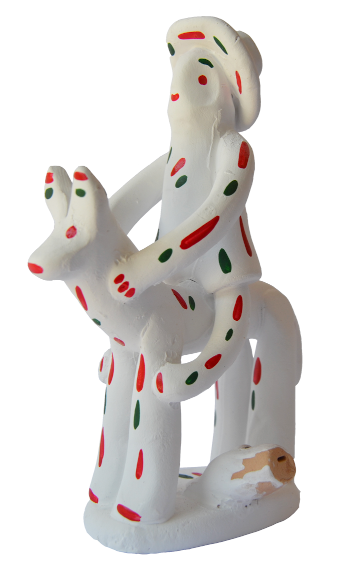
\includegraphics[width=0.3\textwidth]{siurellp}
\caption{\label{fig:siurell}Figura de cerámica\ldots}
\end{figure}

\section{Añadiendo una tabla}

\begin{table}[H]
\centering
\begin{tabular}{|l|c|c|r|}
\hline
\multicolumn{1}{|c|}{Nombre} & Apellido & Edad & \multicolumn{1}{c|}{\begin{tabular}[c]{@{}c@{}}Estudios/\\ Trabajo actual\end{tabular}} \\ \hline
Jesús & Mudarra & 28 & Máster en Ingenería Industrial \\ \hline
Javi & Comes & 26 & Auxiliar de enfermería \\ \hline
Andrea & Lloret & 26 & Hostelería \\ \hline
Álvaro & Valcárcel & 27 & Grado en Ingeniería Informática \\ \hline
\end{tabular}
\caption{Lista de amigos}
\label{tab:my-table}
\end{table}

\newpage

\section{Haciendo referencia a la bibliografía}

\citet{Brooks1997Methodology}
demuestra que \ldots\\

Evidentemente, todos los números impares son primos \citep{Jacobson1999Towards}.\\

Dos formas de citar referencias serían:\\
\citep{Smith1990Enabling} o \citet{Smith1990Enabling}

\bibliographystyle{plainnat}
\bibliography{references}

\end{document}